\section{The world and the machine}

\begin{center}
	\vspace{0.2cm}
	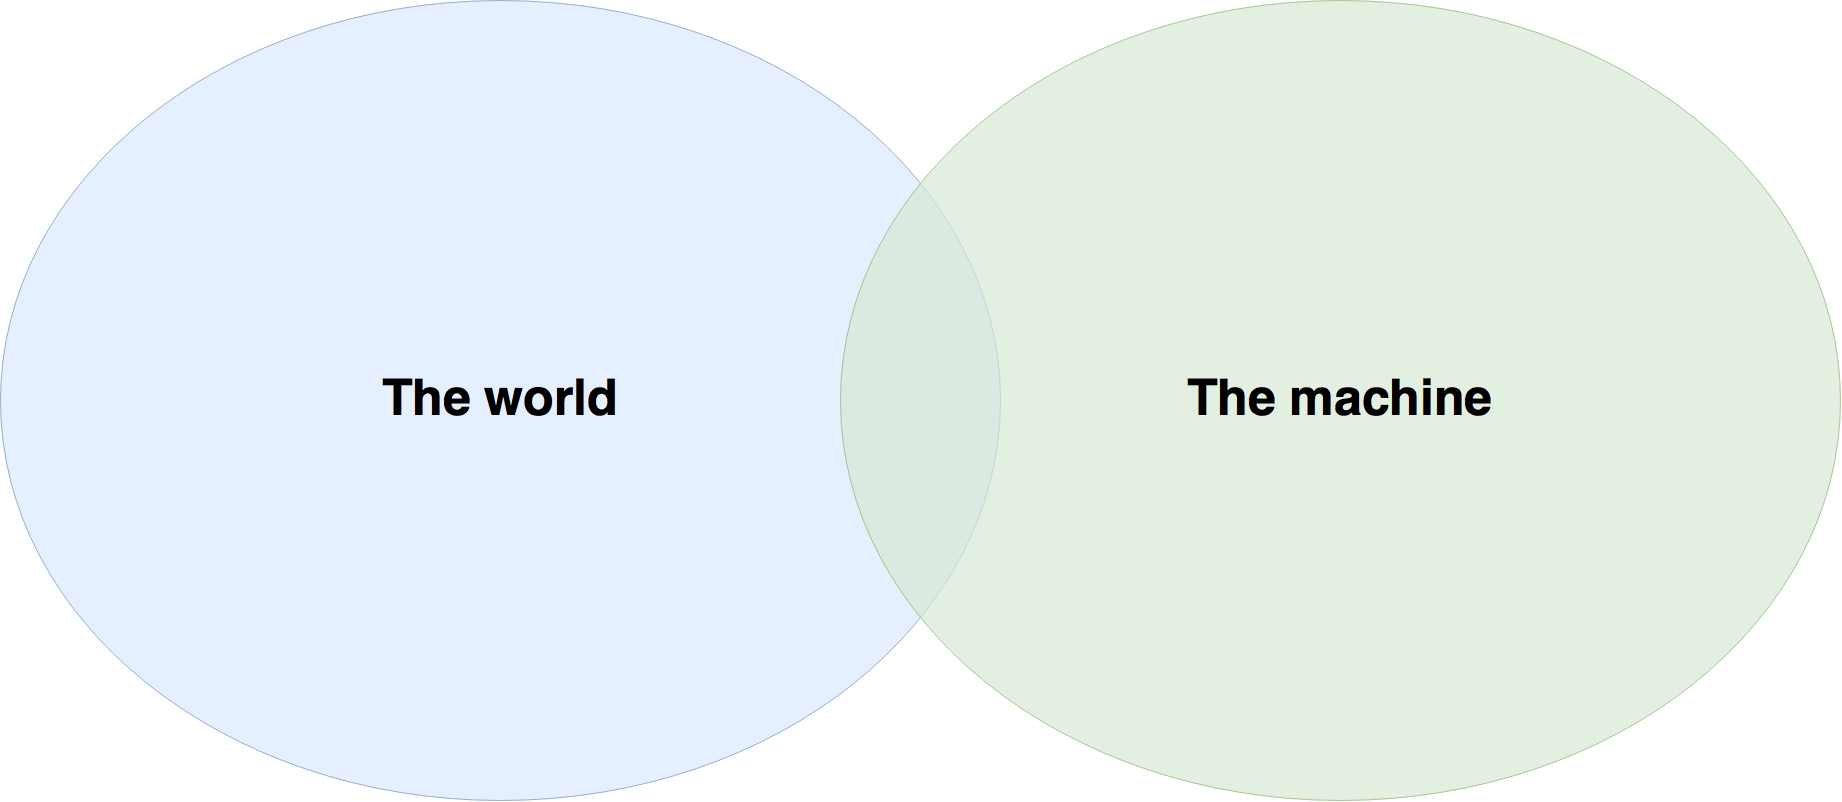
\includegraphics[width=0.50\textwidth]{/RASD/TheWorldAndTheMachine}\\ 
	\vspace{0.5cm}
\end{center}


\section{Scenarios}

\section{Use cases}


\subsection{Guest}


\subsubsection{Log-in}

\begin{center}
  \begin{tabular}{ l | p{10cm} }
    \hline
    \textbf{Name} & \textbf{Log-in} \\ \hline
    Actors & Guest\\ \hline
    Entry conditions & 
\begin{itemize}
\item The Guest has to be sucessfully registered to PowerEnJoy.
\item The Guest entres the Log-in page in the browser/ mobile application. 
\end{itemize} \\ \hline
    Flow of events &
\begin{itemize}
\item The Guest insert her \gls{ID} and \gls{pwd}.
\item The Guest clicks the Log-in button.
\item The system loads the User's homepage.
\end{itemize} \\ \hline
  	Exit conditions & The User is in the PowerEnJoy homepage. \\ \hline
	Exceptions & 
\begin{itemize}
\item The Guest provides wrong username-password pair (the system signals a LoginError).
\item The Guest doesn't fill both the fields (the systems signals an InformationLack).
\item The system is not able to complete the operation due to some internal issues or connection broken (the system signals a CennectionToSystemFail).%volendo si possono modificare i nomi delle eccezzioni.
\end{itemize} \\ \hline
  \end{tabular}
\end{center}

\subsubsection{Registration}

\begin{center}
  \begin{tabular}{ l | p{12cm} }
    \hline
    \textbf{Name} & \textbf{Registration} \\ \hline
    Actors & Guest\\ \hline
    Entry conditions & 
\begin{itemize}
\item The Guest has to have internet access.
\item The Guest entres the Sign-up page in the browser/ mobile application. 
\end{itemize} \\ \hline
    Flow of events &
\begin{itemize}
\item The Guest is shown a form to fill with her personal e-mail, name, surname, tax code and phone number. %da scegliere se l'ID viene scelto dal system o dal Guest 
\item The Guest fills the form and confirm her provided information.
\item The Guest is shown a form to fill with her drive license's information.
\item The Guest fills the form and confirm her provided information.
\item The Guest is shown a form to fill with her payment information.
\item The Guest fills the form and confirm her provided information.
\item The system sends a confirmation e-mail to the Guest's personal e-mail with an activation link.
\item The Guest clicks the link in the system's e-mail.
\item The system allocates the User in the database.
\item The system sends an e-mail to the User's e-mail with her personal \gls{pwd}.
\item The system loads the User's homepage.
\end{itemize} \\ \hline
  	Exit conditions & The Guest is registered to PowerEnJoy and became an User. Now the User is in her homepage. \\ \hline
	Exceptions & 
\begin{itemize}
\item The Guest provides an e-mail or a phone number or a tax code already used (in this case the system signals an error).
\item The Guest does not fill one or more fields in a form (in this cases the system does not allow to proceed and signals an InformationLack).
\item The Guest provided wrong payment information (in this case the system signals an error).
\item The Guest provided wrong drive license information (in this case the system signals an error).
\item The system is not able to complete the operation due to some internal issues or connection broken (the system signals a CennectionToSystemFail).%volendo si possono modificare i nomi delle eccezzioni.
\end{itemize} \\ \hline
  \end{tabular}
\end{center}